\section{Evaluation and Results}
\label{sec:evaluation-and-results}

We seek to evaluate whether \textsc{Appjudicator} is able to successfully
achieve its goal of distinguishing user-initiated network flows using UI
context, and whether it can do so with acceptable overhead. To determine whether
the app accomplishes its goal we perform a practical analysis and to measure the
app's resource cost we perform a performance evaluation. We now explain the
procedures used for each of these experiments and their results.

\subsection{Differentiating User-generated Flows}
\label{sec:differentiating-user-generated-flows}

The goal of this experiment is to determine whether \textsc{Appjudicator} can
successfully distinguish between network flows that were specifically initiated
by a human user and flows generated automatically by an app or the Android
system.

\subsubsection{Experimental Setup}
\label{sec:experimental-setup}

For this experiment, we tested the app both in an emulator an on a physical
Android device. The emulator test was performed on a virtual Google Pixel 4,
with API level 30 (the newest available). Physical tests were performed on a
real Google Pixel 3 phone running Android 11 with API level 30.

In both cases we used Google's UI Automator framework~\cite{uiautomator2020} to
automate the testing process. This tool is designed for automating UI tests as
part of an app development cycle, and provides features that make it ideal for
our experiments. The UI Automator can simulate various kinds of UI interactions,
including clicks, swipes, pressing hardware buttons, and even changing the
device's orientation. It can also perform actions in multiple apps in a single
run.

We use UI Automator to simulate a series of real life use cases that would lead
to a network request being made while \textsc{Appjudicator}'s accessibility
service is enabled. Then we simply check service's logs to see which flows it
marked as likely user-initiated. We run the test $x$ times to make sure the
results are reproducible, and not merely a coincidence of timing. See
Section~\ref{sec:practical-results} for the results of this experiment.

\subsubsection{Results}
\label{sec:practical-results}

% Use UI Automator to simulate real clicks, also find other apps that make background requests automatically
% Log whether each flow was user-generated, default-allowed, or automated
% What percentage of those flows were classified successfully?

\subsection{Performance Evaluation}
\label{sec:performance-evaluation}

To fulfill its purpose as an always-enabled enterprise network security tool,
\textsc{Appjudicator} has to be as unobtrusive to end users as possible. This is
especially important because the app performs some actions on every network
flow, so any latency added by it would be especially noticeable.

\subsubsection{Measuring Added Latency}
\label{sec:measuring-added-latency}

To measure the effect of \textsc{Appjudicator} on network communication speed,
we measure the total additional latency added by the app when initiating a TCP
connection.

For this test, we run the app in an Android virtual machine simulating a Google
Pixel 4, on API level 30. We use POX's \texttt{forwarding.hub} module as an
OpenFlow controller. In this mode, the controller responds to every query with
an instruction to forward the flow to its destination~\cite{mccauley2015}. Local
network latency is not a part of this test, so the controller server runs on the
same physical host as the Android virtual machine. The two components still
communicate over a regular TCP connection. The SDN agent starts with an empty
table of flow rules, so it must send a \texttt{packet\_in} to the controller for
every new flow. See Section~\ref{sec:openflow-protocol} for more information
about the OpenFlow protocol.

We measure the added latency of the first packet in a TCP connection because
this is where the system does the most processing. The start of a new flow
requires an SDN agent flow table lookup and possibly communication with the SDN
controller, and the app has to do more processing for TCP connections than UDP
connections. Subsequent packets in a TCP flow, and all packets in UDP flows
have lower latency.

We configure the app to log a timestamp when an outgoing TCP SYN packet is
intercepted from the device. \textsc{Appjudicator}'s VPN service then queues the
packet and asks the SDN agent what to do with it. The SDN agent tries to look up
the flow in its flow table and, finding no matching entry, sends a
\texttt{packet\_in} message to the controller. After the POX controller responds
with a \texttt{packet\_out} the SDN agent tells the VPN service to forward the
queued packets in the flow. Just before the initial SYN packet is sent to the
network a second timestamp is recorded. The earlier timestamp is the time the
packet would have been sent to the network without \textsc{Appjudicator}'s
influence, so the difference of these two timestamps is the total latency added
by the app.

There were 562 measured TCP connections during the sampling period and seven
removed as outliers, leaving 555 data points. The average added latency was 138
milliseconds, with a standard deviation of 38 milliseconds. In our sample 97\%
of TCP connections started with less than 200 milliseconds of added latency.
Figure~\ref{fig:tcp-delay-chart} charts the full results.

\begin{figure}[h]
    \centering
    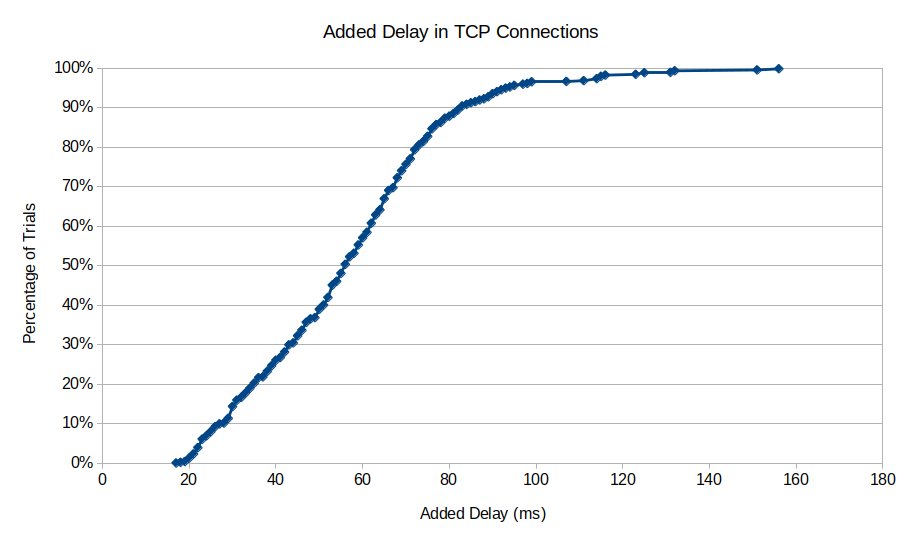
\includegraphics[width=\textwidth]{tcp-delay.png}
    \caption{Total latency added when initiating new TCP connections.}
	\label{fig:tcp-delay-chart}
\end{figure}

\subsubsection{Measuring Resource Overhead}
\label{sec:measuring-resource-overhead}


\newpage
